\documentclass[letter]{report}
% change draft to final when ready
% letter is US paper size 8.5 x 11.0 inches (215.9 x 279.4 mm)
% a4 is India/Europe 210 x 297 mm size

\newcommand\thesisTitle{MTech Thesis [Drafts] Template for AmritaU}
% title  of *your* thesis in Title Case

\usepackage[final]{graphicx}
% keep final to render figures; use draft to just have rectangles

\usepackage[usenames,dvipsnames]{color}
\PassOptionsToPackage{hyphens,obeyspaces,spaces}{url}
\usepackage{hyperref}
\hypersetup{
    pdftitle={\thesisTitle},
    pdfauthor={www.wright.edu/\~pmateti},
    pdfsubject={Latex and Theses},
    pdfkeywords=Latex and Theses,
    pdfcreator={emacs},
    pdfproducer={pdflatex},
    pdfnewwindow=true,
    colorlinks=true,        % false: boxed; true: colored
    linkcolor=blue,
    citecolor=Brown,
    filecolor=blue,
    urlcolor=Brown,
    bookmarks=true,
    unicode=false,
    pdftoolbar=false,
    pdfmenubar=false,
    pdffitwindow=true,
    pdfstartview={FitH},
}
\usepackage{algorithm2e}
\usepackage[square]{natbib}

% helpful macros while writing drafts of the proposal/ thesis
\newcommand\TBD[1]{\textcolor{red}{TBD~~#1}}
\newcommand\TBDMP[1]{{#1}\footnote{To be rewritten more precisely.}}
\newcommand\TBDMTBW{\quad More to be written.}
\newcommand\TBDFIG{{\vskip 2in}\footnote{Insert a figure here.}}
\newcommand\bumppages[1]{\addtocounter{page}{#1}}
\newcommand\KeepButNotInclude[1]{}

\newcommand\singleSpacing{\def\baselinestretch{1.0}}
\newcommand\doubleSpacing{\def\doubleSpacing{\def\baselinestretch{1.37}\normalsize}}


% LaTeX macros specific to this template example
\newcommand\TEX{\TeX{}}
\newcommand\tex{\TeX{~}}
\newcommand\web{{\tt WEB }}
\newcommand\latex{\LaTeX{~}}
\newcommand{\bibtex}{BiBTeX{~}}

\begin{document}

\pagestyle{plain}\newpage\pagenumbering{roman}\setcounter{page}{1}



\thispagestyle{empty}


\begin{center}

{\bf\Huge
Typesetting a Thesis/ Dissertation\\
Using Mateti's {\LaTeX} Example\\ %% title
}
\par\vskip 4cm

(\TBD{} For {\it this} document, the following is NOT true.)\\
A thesis submitted in partial fulfilment\\
of the requirements for the degree of\\
Master of Science in Computer Engineering\\  % replace

\par\vskip 2cm
By\\
\par\vskip 2cm


PRABHAKER MATETI\\              %% author name, all caps
B.S., Osmania University, 1970\\        %% previous degrees
M.Tech., Indian Institute of Technology at Kanpur, 1972\\
Ph.D., University of Illinois at Urbana-Champaign, 1976\\


\vfill

2016\\                          %% Year
Wright State University\\
Dayton, Ohio 45435-0001\\


\end{center}

\newpage


\newpage
\thispagestyle{empty}

\begin{center}
AMRITA SCHOOL OF ENGINEERING \\
AMRITA VISHWA VIDYAPEETHAM\\
\end{center}

\hfill
July 25, 2017\\			% DATE OF DEFENSE

I HEREBY RECOMMEND THAT THE THESIS PREPARED UNDER MY SUPERVISION BY
{\tt Sudip Hazra}		%% Full Name of the Student
ENTITLED
{\tt \thesisTitle}
BE ACCEPTED IN PARTIAL FULFILLMENT OF THE
REQUIREMENTS FOR THE DEGREE OF
{\tt Master of Technology in Cyber Security Systems and Networks}.\\


\hfill
\begin{minipage}{7cm}
\vskip 1cm\hrule\par\vskip 2mm
Prabhaker Mateti, Ph. D.\\	%%
Thesis Director\\
\vskip 1cm\hrule\par\vskip 2mm
Krishna Sri Achuthan, Ph.D.\\
Department Head\\
\end{minipage}

\vfill
\begin{minipage}{7cm}
Committee on\\
Final Examination\\
\vskip 1cm\hrule\par\vskip 2mm
Prabhaker Mateti, Ph. D\\
\vskip 1cm\hrule\par\vskip 2mm
Professor B, MTech or Ph. D\\
\vskip 1cm\hrule\par\vskip 2mm
Professor B, MTech or Ph. D\\
Professor C, MTech or Ph. D\\
\vskip 1cm\hrule\par\vskip 2mm
Krishna Sri Achuthan, Ph.D.\\
Dean, School of Graduate Studies
\end{minipage}

\newpage
\thispagestyle{plain}

{\centering\bf ABSTRACT\\}\par\vskip 2cm

\singleSpacing
\noindent
Subramanian, Sripriya.          %% last, first name, upper-lower case mix
M.S.  Department of Computer Science and Engineering,
Wright State University,
2003.                           %% this year
Sniffing the Ethernet with High Quality Tools. %% title

\par\vskip 2cm

\doubleSpacing

[This document is an example collection of files intended to help my
students in using LaTeX as they prepare their theses.  An abstract is
typically about one page.  The following is an example of an abstract
of a thesis.]

This thesis is a study of software quality in the limited context of a
class of network software tools called {\em sniffers}. Sniffers are
network monitoring tools used in the administration of network
security. We analyzed five of the hundreds of the existing sniffers to
determine the causes of poor quality and the methods to eliminate the
problems. We subjected the five selected sniffers to both manual
analysis and analysis by software quality assessment tools. We
classify the 1000+ errors so discovered in these sniffers. Based on
these results, we designed and implemented a new sniffer that is
intended as a model of high quality sniffer. The methods applied to
analyze and enhance the quality of software are studied.

Quality assessment software tools fall into two categories: 1) Static
checkers and 2) Dynamic checkers. Static checkers analyze the source
code. Dynamic checkers stand as guards during run-time. We have
collected and used exhaustively the checker tools that are in the open
source archives. In the course of our use, the quality of the software
quality tools is itself analyzed.

This thesis contributes several case studies of open source software
projects. It also contributes a new distributed sniffer to the open
source. The distributed sniffer can monitor multiple networks and
output desired packet details. We designed our sniffer to include a
MySQL based collector program, packet capture programs and viewer
programs. Our sniffer supports multiple capture and viewer
programs. We applied software engineering methods to eliminate the
quality issues associated with software. We use the results of our
analysis of existing sniffers in avoiding poor quality in our
sniffer. We prepared our sniffer for manual audit using documentation
tools. This new sniffer is an example of {\it literate programming}
that is worthy of study by software engineering students.

\newpage





\tableofcontents
\listoftables
\listoffigures
\newpage
\thispagestyle{plain}

{\centering\bf  ACKNOWLEDGEMENTS\\}\par\vskip 2cm

\singleSpacing
\noindent


\noindent
At the very outset, I would like to give the first honors to Amma, Mata Amritanandamayi
Devi who gave me the wisdom and knowledge to complete this minor project under her shelter
in this esteemed institution.
I express my gratitude to my guide, Prof. Prabhaker Mateti, Associate Professor, Com-
puter Science and Engineering, Wright State University, USA, for his valuable suggestion
and timely feedback during the course of this minor project.
I would like to thank Dr Krishnashree Achuthan, Professor and Head of the Center for
Cyber Security, for giving me useful suggestions and his constant encouragement and guidance
throughout the progress of this minor project.
I would like to thank my co-guides Mr. Vipin Pavithran, Assistant Professor, Cyber Secu-
rity, Amrita Vishwa Vidyapeetham for giving me useful suggestions and guidance throughout
the progress of this minor project.
I express my special thanks to my colleagues who were with me from the starting of the minor
project, for the interesting discussions and the ideas they shared. Thanks also go to my friends for sharing so many wonderful moments. They helped me not only enjoy my life, but also enjoy
some of the hardness of this minor project.

\vfill

\noindent


\doubleSpacing

\newpage





\pagestyle{headings}\newpage\pagenumbering{arabic}\setcounter{page}{1}

\chapter{Introduction}

I want all my students to typeset their work using \LaTeX{}.  To
reduce their effort in doing this, I give this report and the
accompanying \LaTeX{} files as an example to learn from.  The details
of \LaTeX{} as used in these example files is sufficient to most of
their documents.

\section{Advice}

\begin{quote}
{\hfill{}``Down with MS Word. Long live \LaTeX.}''  
\end{quote}

\noindent
This is the underlying sentiment in this article.

I recommend various things below without justifying them.  This keeps
the article short.

\section{``I say so.''}

Besides, I have some dictatorial powers over my students ``{\tt
  ;-)}''.  And, these are CS students.  They are supposed to be able
to learn new languages and tools fast!  No?

\section{Length}

There are really no rules about the length of a chapter.  But should a
chapter be this short?

% -eof-

\chapter{Mateti's {\LaTeX} Thesis Example}

I recommend that you use my collection of
files\footnote{\url{http://www.cs.wright.edu/~pmateti/Students/thesisExample.tbz}}.
My own contribution here is not original.  It is in pulling together
various needed pices in trying to reduce the \LaTeX-learning time for
my students.

\section{Contents of the {\tt tar} File}

The downloaded file is a {\tt tar} archive compressed with {\tt
  bzip2}.  You can untar it, in Linux, as in

{\tt tar xvfj thesisExample.tbz}

Your current directory will then have a new subdirectory called
ThesisEx/ with the following files and subdirectories in it.
[Ignore the dates, and usernames.]

\begin{verbatim}
drwxr-xr-x    2 pmateti  pmateti      4096 May 24 13:07 Chapters/
drwxr-xr-x    2 pmateti  pmateti      4096 May 24 11:44 Figures/
drwxr-xr-x    2 pmateti  pmateti      4096 May 24 11:44 LaTeX/
-rw-r--r--    1 pmateti  pmateti       713 May 24 11:47 Makefile
drwxr-xr-x    2 pmateti  pmateti      4096 May 24 13:09 Tables/
-rw-r--r--    1 pmateti  pmateti      8513 May 24 11:44 thesis.bib
-rw-r--r--    1 pmateti  pmateti      1158 May 24 11:47 thesis.tex
drwxr-xr-x    2 pmateti  pmateti      4096 May 24 11:44 WSU/
drwxr-xr-x    2 pmateti  pmateti      4096 May 24 11:44 AmritaU/
\end{verbatim}

\section{Your Use of these Files}

The files in the directory LaTeX are to be left as they are.  Note the
content of file named {\tt thesis.tex} from the very top to the line
\verb|\begin{document}|.  Edit these only if you are fluent in LaTeX.

Edit the files in the WSU or AmritaU directory to insert your own name,
etc.

Replace all the files in the {\tt Chapters/ Figures/ Tables/}
directories with yours.  Edit the {\tt thesis.tex} to input the files
in the {\tt Chapters/ Figures/ Tables/} directories.

Use the given {\tt Makefile} as a template and adjust.

This example template of a manuscript is written in the style of
learn-by-example.  The text body (in the pdf) shows what is possible,
and you are expected to study the \latex{} source of these chapters to
learn how things were done.

\section{Bib Files}
\label{BibFiles}

If you have several .bib files, move them into a {\tt BiB/} directory.
Note that \verb|\bibliography| does accept multiple filenames
(pathnames), separated by commas, but no spaces.  E.g., {\tt
  \verb|\bibliography|\{Bib/amrita, ..., Bib/cloud-comp,
  Bib/cloud-storage, Bib/code-audit, Bib/crowd-source, Bib/forensics,
  ..., Bib/malware, Bib/privacy, Bib/provenance,
  Bib/zygote-aslr-rop\}} is {\sc ok}.  Make sure there are no spaces,
and no ellipses -- I included these here just for readability.

% -eof-

\chapter{Technical Report Writing}

A thesis is a technical report.  Read and follow a good style book
(e.g., Chicago) on technical report writing.  It is a good exercise to
mark {\em this} article up!  Additionally, every university has
guidelines regarding layouts and required pages such as a title page
an approval page.

(This article is itself poorly and hastily written.  Think of it as a
collection of notes.  ``Do as I say, not as I do! {\tt ;-)}'' )


\section{Order and Content of the Chapters}

This chapter is about the ordering of academic/technical content.  I
am particularly annoyed by the ``wrong order'' of chapters.  I
recommend the following order for the chapters.  But, do choose better
titles than the generic ones I am using below.

\begin{description}
\item[Abstract]

  Of course, Abstract is not a chapter!  In a technical report, the
  Abstract should be a summary of the contents.  Too many published
  papers include motivational sentences, and even citations.  These
  are inappropriate.  Typical length of a thesis abstract is a page.  

\item
  [Introduction] should restate the abstract, preferably using
  different sentences.  It is customary that the last paragraph
  describes the structure of the report.

\item
  [Background] describe concepts and terminology needed to understand
  the rest.  There should always be a chapter (in a thesis) or a
  section (in a paper) on backround.  This is a collection of
  definitions and (extremely brief) tutorials on what the reader
  should know in order to appreciate the main body of your tech
  report.  The length of this should never exceed, say, 1/10 of the
  tech report.  In a thesis, this is almost always the second chapter.

\item
  [Problem Statement] should be rigorous, and complete.  Also address
  the following: Why is it interesting to solve? Is it too trivial and
  not at the MTech/PhD level? Is it too hard to solve?  ``Problem
  Statement'' is a poor title -- choose better.

\item [Architecture and Design]
  Details of (Your) Solution. This may be multiple chapters.

\item [Related Work] There should always be a chapter (in a thesis) or
  section (in a paper) on related work.  This is an organized critique
  of the body of literature related to the work you are doing.  The
  expectation is that this is exhaustive.  What have others done?  Do
  summarize, but focus on critiquing.  This is not a collection of
  paragraphs summarizing individual papers.  It is almost always a bad
  idea to make this the second chapter.

  Place this chapter after a discussion of your work.  Then, you will
  be able to compare your work with that of others.    Discuss your
  dependencies -- what you are using from where?  This chapter (almost
  always) should follow your solution so that you can discuss
  comparatively your decisions in your solution.

\item
  [Discussion] of Alternatives (what else could have provided answers).

\item
  [Evaluation] of Your Solution (qualitative as well as quantitative).

\item
  [Conclusion] Use it with both of its meanings: deductions, and
  finishing.

\item
  [References] Must be ``properly'' done.  See the Section
  \ref{References}.


\end{description}

\section{Structure}

When you are moving from a chapter heading to its first section, and
from a section heading to its first subsection there is always an
introductory paragraph.

Sometimes we like to write a paragraph at the end of a chapter that
does not belong to the last section.  This is often done by
introducing some extra vertical white space after the end of the last
section that is longer than the typicial spacing between consecutive
sections.

There are no particular size requirements.  But, a one page chapter
and a two line section do look silly.

\section{URLs}

URLs are now common in CS theses.  Older style guides do not cover
these.  Include a URL inside \verb|\url{}|. Example:
\url{http://www.google.com/search?q=latex+eepic+pstricks+tikz}
The package named {\tt hyperref} has a macro named \verb|href| with
two arguments: first one, a URL, second one, the text to be displayed.


\section{Acronyms}

Acronyms are written in all-upper case.  Examples: {\sc gnu}, {\sc
  bcpl}, {\sc kde}.  Linux, Unix, Android, Scala, Java, ... are not
acronyms.  Do not write LINUX; change it to Linux, no boldface, L in
caps, the rest in lower case.

\section{References}
\label{References}

Use BiBTeX.  The file named {\tt thesis.bib} should contain the
references you collected in the {BibTeX} syntax.  I have included a
few references to illustrate this syntax; you can leave them in this
file.  In general, it can contain many more references than what you
cite in the body of your thesis.  The {\tt bibtex} program examines
the actual citations made, and pulls together the cited references
into the text file named {\tt thesis.bbl}.  See also Section
\ref{BibFiles}.

Pay attention to the complaints of {\tt bibtex}.  Publication venue
(conference or journal), year, and page numbers of the paper are a
must.  Include {\sc url} of the paper ({\sc html} or {\sc pdf}), if
available.

Bibliographic citations are done in many ways.  I prefer [Author-Name,
  Year] style.  This report used {\tt
  \verb|\bibliographystyle|\{Bib/acmtrans\}}, a style that
ACM\footnote{\url{http://www.acm.org/}} Transactions use.  Other
acceptable choices are those that include author(s) last name and year
of publication in the body of the text that cites, and the end of the
article list of references are sorted alphabetically by the first
author's last name.  Styles that produce a bracketed number, as in
[5], are not acceptable to me.

When using \url{http://scholar.google.com/}, set Bibliography Manager
to use BibTeX in the preferences.  Then, the references found
can be saved in \bibtex{} format.  Visit also
\url{https://www.mendeley.com/},
\url{http://bibsonomy.org/} and \url{http://zotero.org}.

\section{Plagiarism}

Using someoneelse's work without crediting them is plagiarism.  There
are many software tools and web services that can pinpoint lifted
sentences.  Quoting is ok, but must always use double- or sigle-quotes
and cite immediately.

% -eof-

\chapter{Routine Use of {\LaTeX} }

Most documents contain forward references to \verb|\label|s.  So, often we
must latex the files twice.

\section{Document Structure}

The macro \verb|\chapter| is self-explantory.  These also introduce a
line in the table of contents (.toc) file.  The .toc file is generated
at the end of LaTeX processing.  So, to include a table of contents
properly at the beginning of the document, we must {\tt pdflatex} the
files twice.

The depth of sections that show up in the TOC is typically set in the
report style to 3.  You can change this, to say 9, by including the
line\\ {\tt \verb|\setcounter|\{secnumbookdepth\}\{9\}} in {\tt thesis.tex}.

\section{Lists}

LaTeX has three kinds of lists.  Description list is often better than
{\tt enumerate} which is better than {\tt itemize}.

\section{Figures}

Figures and tables float, often ending up at the top of a page, or
even at the end of the document.  To control this, learn the
\verb|!htb| options of the {\tt figure} environment.  
Figures should be no more than a single page; rework them if
they are not.

Each of the \TeX/ \LaTeX{} specific packages {\tt eepic}, {\tt
  pstricks}, {\tt graphicx}, and {\tt tikz} is capable of producing
intricate drawings, but the learning curve is steep.
You must explore the collection of figures at
\url{www.texample.net}.

\subsection{\LaTeX{} File Genreated by {\tt xfig}}

Figure \ref{trie} was interactively drawn using {\tt xfig} and then
exported as a .tex file from it.  Typcially, we \verb|\label| the
figures so we can reference it.  Look at the source \LaTeX{} file of
this chapter.

\begin{figure}[ht]\centering
\setlength{\unitlength}{3947sp}%
%
\begingroup\makeatletter\ifx\SetFigFont\undefined%
\gdef\SetFigFont#1#2#3#4#5{%
  \reset@font\fontsize{#1}{#2pt}%
  \fontfamily{#3}\fontseries{#4}\fontshape{#5}%
  \selectfont}%
\fi\endgroup%
\begin{picture}(5787,3030)(751,-3586)
\thinlines
\put(4726,-1486){\vector(-1, 0){2625}}
\put(5326,-1486){\vector(-1, 0){375}}
\put(1951,-1636){\vector( 3,-1){2475}}
\put(3826,-736){\vector( 4,-1){2700}}
\put(2776,-2611){\vector(-1, 0){1425}}
\put(4276,-2611){\vector(-1, 0){1200}}
\put(1276,-3511){\vector(-1, 0){225}}
\put(2551,-3511){\vector(-1, 0){300}}
\put(3076,-3511){\vector(-1, 0){300}}
\put(3676,-3511){\vector(-1, 0){225}}
\put(4426,-2761){\vector( 0,-1){675}}
\put(3001,-2761){\vector( 3,-2){900}}
\put(1201,-2761){\vector( 1,-3){225}}
\put(1726,-1561){\makebox(0,0)[lb]{\smash{\SetFigFont{12}{14.4}{\rmdefault}{\mddefault}{\updefault}a:16}}}
\put(4801,-1561){\makebox(0,0)[lb]{\smash{\SetFigFont{12}{14.4}{\rmdefault}{\mddefault}{\updefault}b}}}
\put(5401,-1561){\makebox(0,0)[lb]{\smash{\SetFigFont{12}{14.4}{\rmdefault}{\mddefault}{\updefault}c}}}
\put(5926,-1561){\makebox(0,0)[lb]{\smash{\SetFigFont{12}{14.4}{\rmdefault}{\mddefault}{\updefault}...}}}
\put(3601,-661){\makebox(0,0)[lb]{\smash{\SetFigFont{12}{14.4}{\rmdefault}{\mddefault}{\updefault}root}}}
\put(6526,-1561){\makebox(0,0)[lb]{\smash{\SetFigFont{12}{14.4}{\rmdefault}{\mddefault}{\updefault}z}}}
\put(1051,-2686){\makebox(0,0)[lb]{\smash{\SetFigFont{12}{14.4}{\rmdefault}{\mddefault}{\updefault}n:5}}}
\put(3751,-3586){\makebox(0,0)[lb]{\smash{\SetFigFont{12}{14.4}{\rmdefault}{\mddefault}{\updefault}t:0}}}
\put(2851,-2686){\makebox(0,0)[lb]{\smash{\SetFigFont{12}{14.4}{\rmdefault}{\mddefault}{\updefault}r:0}}}
\put(4351,-3586){\makebox(0,0)[lb]{\smash{\SetFigFont{12}{14.4}{\rmdefault}{\mddefault}{\updefault}e:1}}}
\put(2551,-3586){\makebox(0,0)[lb]{\smash{\SetFigFont{12}{14.4}{\rmdefault}{\mddefault}{\updefault}e:3}}}
\put(3151,-3586){\makebox(0,0)[lb]{\smash{\SetFigFont{12}{14.4}{\rmdefault}{\mddefault}{\updefault}m:1}}}
\put(751,-3586){\makebox(0,0)[lb]{\smash{\SetFigFont{12}{14.4}{\rmdefault}{\mddefault}{\updefault}d:2}}}
\put(1351,-3586){\makebox(0,0)[lb]{\smash{\SetFigFont{12}{14.4}{\rmdefault}{\mddefault}{\updefault}t:1}}}
\put(2026,-3586){\makebox(0,0)[lb]{\smash{\SetFigFont{12}{14.4}{\rmdefault}{\mddefault}{\updefault}c:1}}}
\put(4426,-2686){\makebox(0,0)[lb]{\smash{\SetFigFont{12}{14.4}{\rmdefault}{\mddefault}{\updefault}t:1}}}
\end{picture}

\caption{The figure above is drawn by {\tt Figures/trie.tex} using
  vectors built-in \LaTeX{}}\label{trie}
\end{figure}

You can include an eps or pdf file generated by any drawing tool.

\subsection{JPG and PNG Images}

\begin{table}[htb]
\begin{tabular}{lr}\hline
 \parbox{0.75\textwidth}
         {\TBD{} You can include a .jpg, .png, ...
  file using {\tt includegraphics} while scaling it.  Here we show
  the figure of {\tt Figures/gps-track-line.png}.
  A package named {\tt wrapfig} gives greater control.
}
&
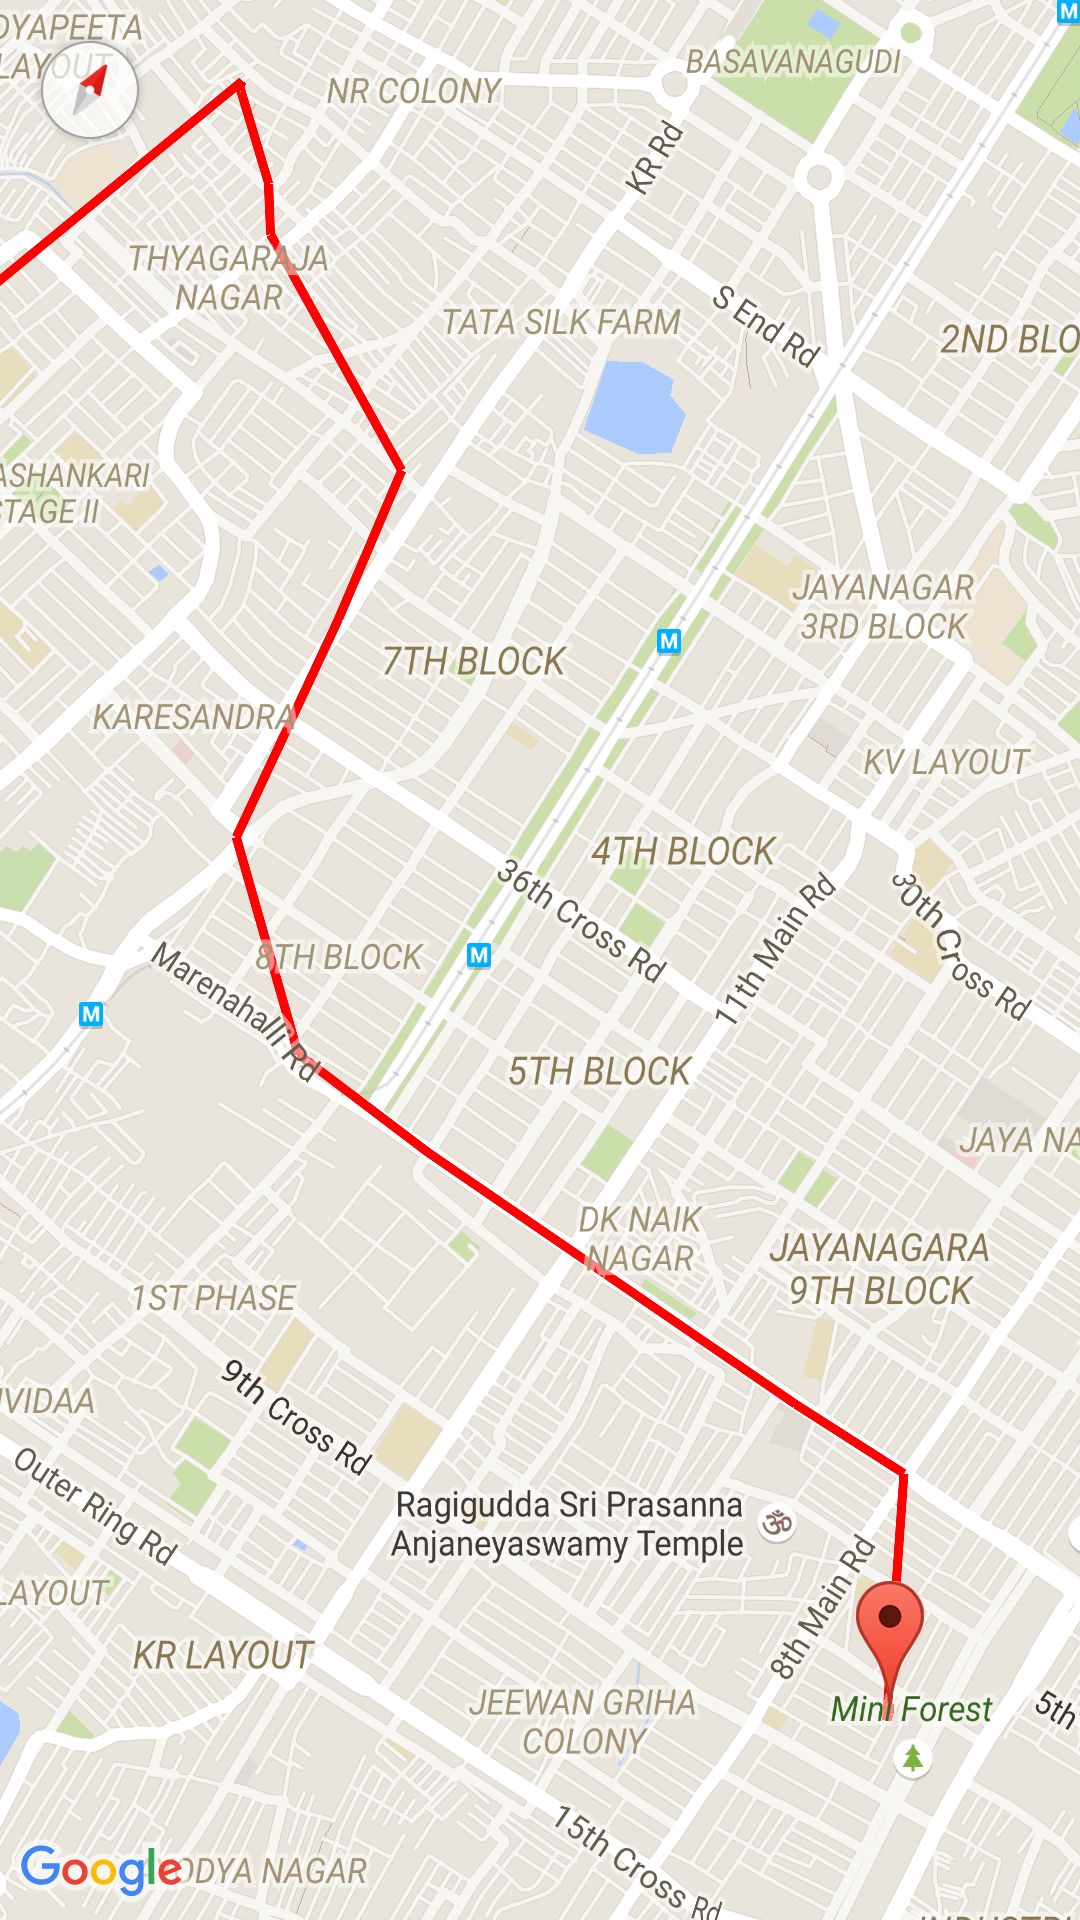
\includegraphics[scale=0.08]{Figures/gps-track-line.png}
\end{tabular}
\caption{This is a table beacuse we used the {\tt table} environment.}
\label{fig:gps-track-line.png}
\end{table}

The ``table'' \ref{fig:gps-track-line.png} is referenced here, and yet
it shows up at the top of the page.  This is known as floating, and we
permitted it by the {\tt htb} options.

\subsection{PDF}

\begin{minipage}{5.0cm}
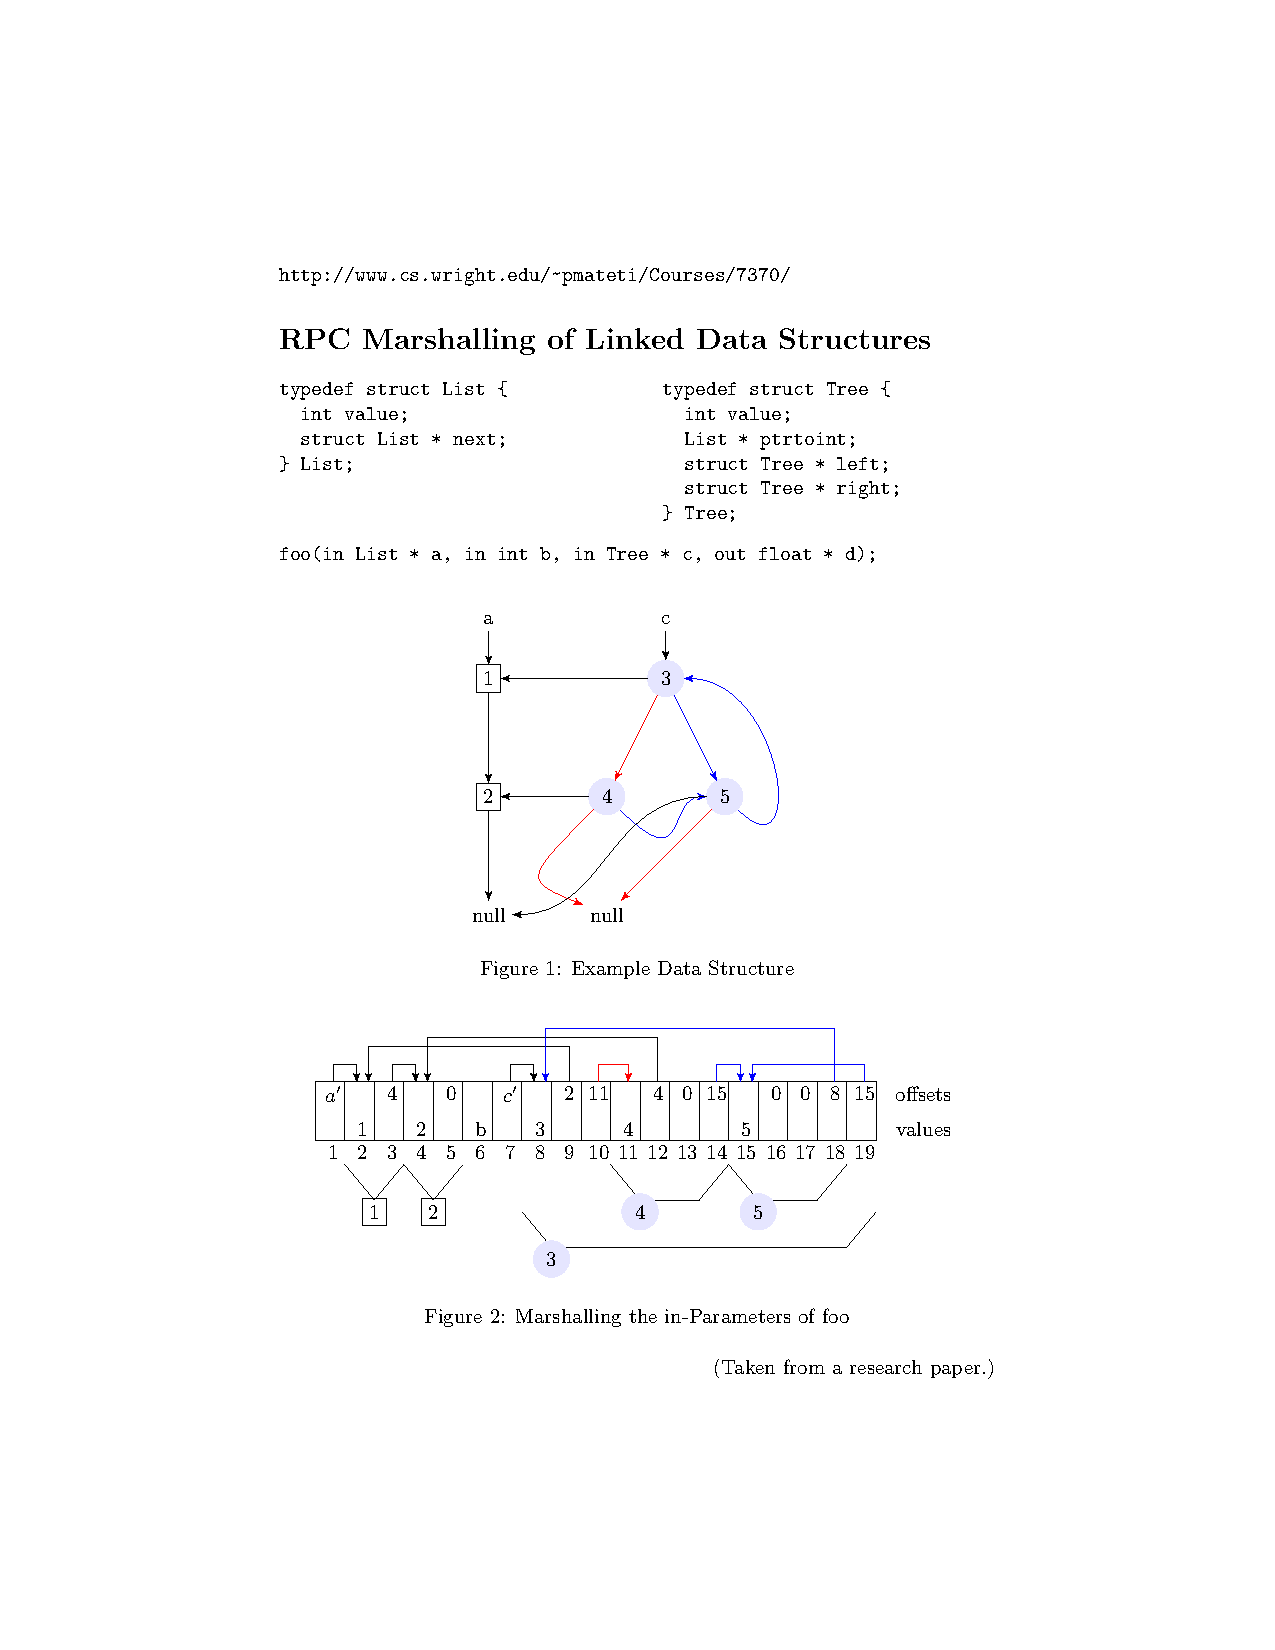
\includegraphics[scale=0.25]{Figures/rpc-marshalling-tikz.pdf}
\end{minipage}
\quad
\quad
\begin{minipage}{5.0cm}
  The left hand figure is produced by {\tt includegraphics \{
    Figures/rpc-marshalling-tikz.pdf \}}.  That is a single page pdf
  with some text and a nicely drawn diagram using TiKZ; click
  \url{./Figures/rpc-marshalling-tikz.pdf} to see it in full size.
\end{minipage}

\subsection{Graphical Plots}

Take your  data, and generate a .png or .pdf file, e.g., using
{\tt gnuplot}.


\section{Tables}

Tables should generally be no more than a single page.  But, if you
must have long tables, look up the packages named {\tt tabularx,
  longtable} and {\tt ltxtable}.

\begin{table}[htb]
\centering
\begin{tabular}{|p{3.75cm}|r|r|r|r|r|}\hline
Category                & {\tt tcpdump} & {\tt sniffit} & {\tt hunt}  &
{\tt dsniff}  & {\tt ethereal} \\ \hline\hline
Word Count & 218455 & 30938   & 45568 & 66599   & 1352372\\ \hline
Lines of Code & 36085  & 3005    & 8817  & 9680    & 280068\\ \hline
Binary Size (Kb) & 488    & 53      & 384   & 482     & 500\\ \hline
Cyclomatic Complexity & 5392   &610      & 2029  & 1517    & na\\ \hline
\end{tabular}


%Actual Binary Size             & 500663 & 54060 & 393700  & 493589  & 3155609 \\ \hline

\caption{Size Summaries of the Selected Sniffers}\label{metric}
\end{table}

\section{Inclusion of Algorithms, ..., Source Code}

Consider ``doing'' literate programming \cite{LP-KNUTH}.

\subsection{Verbatim Mode}

Short pieces of source code can be included in the verbatim mode.  In
this mode, the special characters of \TeX{} are produced as-is.
However, the TAB characters are ignored.  Indentation should therefore
use just blanks.

\begin{verbatim}
#!/bin/bash
# kppp does not correctly set the PPP up.  Here is the fix.
#

fix-ppp() {
    route del -net 0.0.0.0
    route add default gw 130.108.108.8
    route -n
}
\end{verbatim}

For long listings, see \url{en.wikibooks.org/wiki/LaTeX/Source_Code_Listings}.

\subsection{Algorithms}

\newcommand\cupEq{\protect{~\cup{\kern -0.5em}=~}}
\newcommand\plusEq{\protect{~+{\kern -0.5em}=~}}
\newcommand{\OMath}{\ensuremath{\mathcal{O}}}
\renewcommand{\emptyset}{\{\}}
\newcommand\on[2]{{\bf on}{~}{#1}{~\bf do~}{#2}}
\newcommand\bang{{\bf !}~}
\newcommand\query{{\bf ?}~}


\begin{figure}[h]
\begin{minipage}{.45\textwidth}
\begin{algorithm}[H]
  $K_1  := x := 0$\;
  \ForAll {$A \sqsubseteq B \in \OMath_1$} {
    UN \bang update$(B_U, A)$ \query $x$\;
    $K_1 \plusEq x$\;
  }
~\\
  \caption{$A \sqsubseteq B \Rightarrow U[B] \sqsubseteq U[A]$}
  \label{pseudo-R1-2}
\end{algorithm}
\end{minipage}                  % do not insert new lines here
~\textcolor{blue}{\vrule}~
\begin{minipage}{.6\textwidth}
\begin{algorithm}[H]
  $K_2 := x := 0$\;
  \ForAll {$A_1 \sqcap\dots\sqcap A_n\sqsubseteq B \in \OMath_2$} {
    UN \bang $\sqcap(B_U, \{A_1, \dots, A_n\})$ \query $x$\;
    $K_2 \plusEq x$\;
  }
  \label{pseudo-R2-2}
  \caption{{$A_1 \sqcap\dots\sqcap A_n$}
    {$\sqsubseteq B \Rightarrow U[B] \cupEq$}
    {$U[A_1] \cap \dots \cap U[A_n]$}}
\end{algorithm}
\end{minipage}
\caption{Two Algorithms Side-by-Side}
\label{TwoAlgs}
\end{figure}

Figure \ref{TwoAlgs} shows how algorithms can be shown nicely using a
package named {\tt aligorithms2e}; this may need to be installed.  It
created one {\tt figure} using two {\tt minipage}-s.  Several
non-standard math symbols were defined with {\tt newcommand}.
This algorithm is written in pseudo code.

\section{Final v Draft}

The {\tt draft} option is considerably faster than the {\tt final}
when there are many garphical figures.

If you are seeing solid-black rectangles, on some pages, it is because
of the {\tt draft} option in your \verb|\documentclass|.  Change it to
{\tt final}, and these will disappear, but the lines may still stick
out.  Fix these by inserting forced line breaks (usually with
\verb|\\| or \verb|\par|).

% -eof-

\chapter{Learning {\TeX} and {\LaTeX}}

Of course, you {\em should} learn {{\TeX} and {\LaTeX}}!  But, more
importantly you should produce a well-written thesis, that contributes
to existing knowledge, in the time you have.

The files of {\tt thesisExample.tbz} should be enough if you can learn
via examples.

There are many tutorials of varying length, from a few pages to
hundreds of pages; e.g., \cite{WikiBooks}.  The original books are by
\cite{Knuth} who designed and implemented \TEX{}, and \cite{Lamport},
who developed the \LaTeX{}.  ``The Comprehensive TeX Archive Network
\url{http://www.ctan.org/} is the authoritative collection of
materials related to the TeX typesetting system.''

Use {\tt pdflatex} to produce pdf files directly.  Most theses use
{\tt url} and {\tt hyperref} packages\footnote{to produce links such
  as {\LaTeX{} Cheat Sheet} \url{https://wch.github.io/latexsheet/}}.
Note that the LaTeX/pmthesis.cls already includes these.

% -eof-

\chapter{Recommended Software Tools}

Only open-source tools are mentioned in this section.  Only a few
links are given below because they have been changing too rapidly.
Search the web.

\begin{description}

\item[{pdflatex}] directly produces .pdf files.  However, you may wish
  to produce .dvi, then .ps, and finaly .pdf.  DVI-to-PS is by dvips,
  PS to PDF is by ps2pdf.

\item[{qpdfview}], kdvi, xdvi, xpdf, gv, ghostview and okular are for
  previewing.

\item[tetex]There are multiple distributions of \TeX{} and \LaTeX{}
  for Linux.  I used tetex. {MiKTeX} is a complete \TeX{} distribution
  for Windows.

\item[lyx], {\tt texmacs} and {\tt kile} are frontends to \LaTeX{}
  giving a WYSIWIG view.  You might like them.

\item[{emacs}] is excellent for editing TeX files.  There are
  style files for TeX.  Make sure they are loading when you begin
  editing a file with the extension .tex.  Visit
  \url{http://www.emacswiki.org/}.

\item[tikz] Visit \url{http://www.texample.net/tikz/examples/} to see
  the many beautiful, and meticulous, vector drawings.  Steep
  learning.  So is \url{https://inkscape.org/en/}.

\item[xfig] is an old, but still good, GUI tool for vector-based
  drawing.  It can export into \LaTeX{}, eps and other formats.

\item [OpenOffice] and {\tt Inkscape} have vector drawing components
  that are quite good.  They can export into eps or pdf.

\item [{metapost},] {\tt asymptote} are programming languages for
  meticulous drawing.

\item[{graphviz}] is a layout tool for graph theoretic graphs.

\item[{tth}] generates {\sc html} files from your LaTeX files.
  The {tex2page} is better but requires the programming language
  Scheme.

\end{description}

% -eof-

\chapter{Typewriting Conventions}

You will be working with the source files of LaTeX for several months.
So, it is almost as important how the text is laid out in these files
as how good the printed result looks.

\begin{enumerate}
\item
Use Title Case: \url{https://www.google.com/webhp?&ion=1&#q=title+case}

\item
Don't let any line be longer than around 70 chars.  Learn the
``auto-fill'' and LaTeX modes, and ``fill-paragraph'' function of
Emacs.

\item
A comma should never have a preceding blank.  Same with several other
punctuation characters: !;:.\%

\item
Sentences are separated by two blanks.  Emacs can then do
sentence-level editing.

\item
Separate the paragraphs with one empty line.

\item
Section headings should appear by themselves on a line.  Leave two blank
lines above and one below these.

\item
The characters \verb|#&_%[]{}| are special in {\TeX}.  If you must use
them, you have to enclose them in either in the verbatim mode as in
\verb/\verb|#&_%[]{}|/ or provide escape sequences.

\item
In programming opening and closing quotes are the same.  In \LaTeX{},
open quotes are \verb|`| or \verb|``| and the corresponding closing
quotes are \verb|'| or \verb|''|.

\item
It is a good idea to end each of your files with the line \\
\verb|%-eof-|.
\end{enumerate}

% -eof-


\chapter{English}

To most of our students English is not their mother tongue.  A thesis
writer should request some one who is good at English to proof reed
the thesis -- atleast the final draft.  This is not a job of the
advisor/ guide of the thesis.  Request a professor from the English
department to be your reader.

\section{Spelling}

In any technical report, spelling mistakes cannot be forgiven.
We use American spelling.  Watch for: -ise in verbs (should be -ize).
Spell checking LaTeX files can be awkward, but you must.  Doing it
from within Emacs is considerably better.


\section{Misused Words and Phrases}

We can turn a blind eye to an occasional
misuse of (i) the definite vesrsus indefinite article, and (ii) the
singular/plural confusion.

The following are collected from the theses drafts of my students.

\begin{enumerate}

\item Use the upper and lower case properly with names of software,
  etc. E.g., "Java" not "java", "Android" not "android".

\item
  The following words are almost always unnecessary: ``mainly'',
  ``basically'', ``very''.  Grep for each occurrence and remove.

\item
  A comma (almost) always follows the ``e.g.'', whose Latin expansion
  means ``for example''.  The other common abbreviation that we often
  use is ``i.e.'' whose Latin expansion means ``that is.''  Do not use
  i.e.  where e.g. is appropriate.

\item
  The word ``like'' should be replaced with ``such as''.

\item
  ``Softwares''  -- software is itself plural.

\item
  Data is both singular and plural.

\item
  ``less'' versus ``few'': Less is used for ``amorphous'' quantities
  (i.e., real numbers), few is used for discrete items (i.e.,
  integers).

\item
  ``From the top of head'' actually means unthinking.

\item
  ``Implemented'' does not mean ``used'' or ``installed''.

\item
  Latter == the second one, whereas later == (time wise, or ...)
  afterwards.
\end{enumerate}

I strongly urge you to read and heed the advice of the book
\cite{Strunk-and-White}.


% -eof-


% \chapter{\TBD{}}

This ``chapter'' is a list of reminders for my self.  It should not
show up in the pdf, when I am finished with this template.

\noindent
{\huge The very first page.  Bug.  Why is this pdfauthor showing up?
  Do not have time to track this down.  Cut this page out using pdf
  tools. -- pmateti}

usepackage{float}

usepackage[vlined]{algorithm2e} TBD end group at level 1

\verb|###| simple group (level 1) entered at line 1061 ({)
            % delete this line when finished
   
\bibliographystyle{LaTeX/acmtranspm}
\bibliography{thesis}

\end{document}
